%Tamanho da letra/papel/ folha só frente / tipo do documento
\documentclass[12pt, a4paper, oneside]{article}
\usepackage[utf8]{inputenc}
 
\title{The MoveIt! Ultimate Tome of Maximum Knowledge}
\author{Cleber Couto Filho \thanks{funded by the Mandruvah team}}
\date{\today}
%Package pra colocar imagem
\usepackage{graphicx}
\graphicspath{ {images/} }

%Package pra colocar codigo
\usepackage{listings}
\usepackage{color}


\definecolor{dkgreen}{rgb}{0,0.6,0}
\definecolor{gray}{rgb}{0.5,0.5,0.5}
\definecolor{mauve}{rgb}{0.58,0,0.82}

\lstset{frame=tb,
	language=Python,
	aboveskip=3mm,
	belowskip=3mm,
	showstringspaces=false,
	columns=flexible,
	basicstyle={\small\ttfamily},
	numbers=none,
	numberstyle=\tiny\color{gray},
	keywordstyle=\color{blue},
	commentstyle=\color{dkgreen},
	stringstyle=\color{mauve},
	breaklines=true,
	breakatwhitespace=true,
	tabsize=3
}

%Command to one line look like code
\definecolor{light-gray}{gray}{0.95}
\newcommand{\code}[1]{\colorbox{light-gray}{\texttt{#1}}}

%Adiciona a indentação as sections
\usepackage{indentfirst}
\setlength\parindent{24pt}

\begin{document}

	\maketitle
	Esse é um documento feito pela ordem do Mandruvah, com o intuito de proporcionar uma conexão
	com a dimensão do conhecimento robótico, buscando o domínio da ferramenta MoveIt!
	
	\begin{figure}[h]
			\centering
			
\includegraphics[width=0.25\textwidth]{tome.jpeg}
	\end{figure}
		
	\section{Installation}
	Considering that you already have done the full installation of \textbf{ROS Kinetic}, just run:
	
		\begin{lstlisting}
		$ sudo apt-get install ros-kinetic-moveit
		\end{lstlisting}
	Case some packages are missing, just use this form of installation \texttt{ros\--distro\--package\--name} , like:
	
	\begin{lstlisting}
	 $sudo apt-get install ros-kinetic-moveit-commander
	\end{lstlisting}
	
	
	\section{Setup Assistant Tutorial}
	The MoveIt! Setup Assistant is a graphical user interface for configuring any robot for use with MoveIt!. Its primary function is generating a Semantic Robot Description Format (SRDF) file for your robot. Additionally, it generates other necessary configuration files for use with the MoveIt!
	
	
	\subsection{Self-Collision Matrix}
	The self collision matrix disables the collision checking of some pairs of links in order to decrease motion planning time. The sampling density specifies how many random robot positions to check for self collision
		
	\begin{figure}[h]
		\centering
		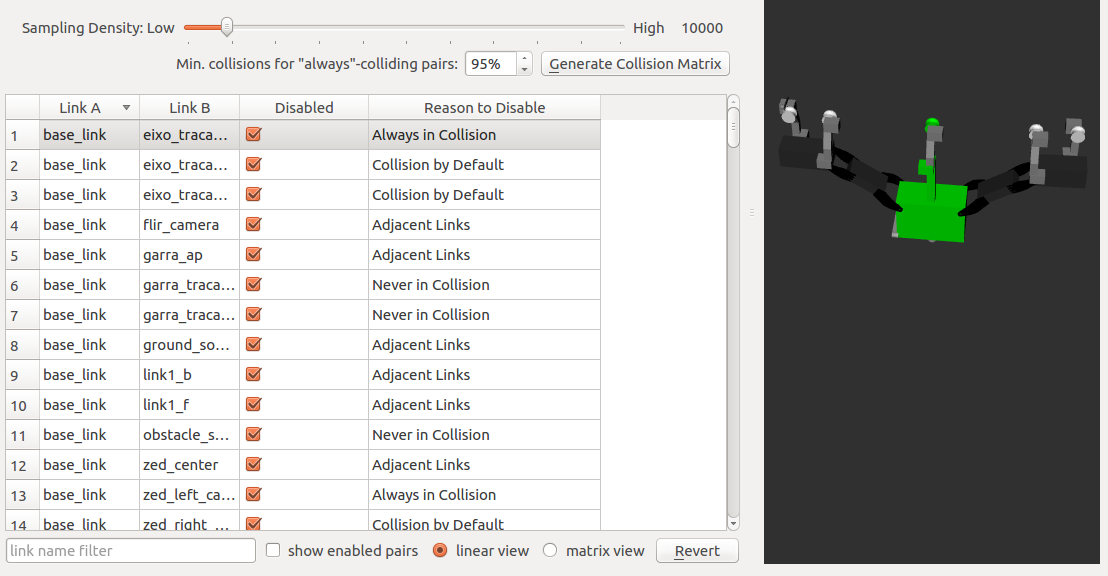
\includegraphics[width=1\textwidth]{self_collision.png}
		\caption{Self-Collision Matrix from Elir Robot}
		\label{fig:collision}
	\end{figure}
	
	
	\subsection{Virtual Joints}
	Used to attach the robot to the world,representing the the motion of the base of the robot in a plane. The parent frame used is the fixed frame of the world.
	
	According to the Rviz tutorial the more-important of the two frames is the fixed frame. The fixed frame is the reference frame used to denote the "world" frame. This is usually the "map", or "world", or something similar, but can also be, for example, your odometry frame.\cite{rviz_site}
	 
	If the fixed frame is erroneously set to, say, the base of the robot, then all the objects the robot has ever seen will appear in front of the robot, at the position relative to the robot at which they were detected. For correct results, the fixed frame should not be moving relative to the world.\cite{rviz_site}
	
	URDF models start with a link at the root, but In MoveIt, models start with a joint. The root joint is the way the robot is connected with the world. The root joint is defined in the SRDF, using the \verb|virtual_joint| tag, and there are 3 types supported right now: fixed(0DOF), planar(3DOF) and floating (6DOF).\cite{moveit}
	
	If there is no virtual joint defined, a fixed one is assumed. The planning frame will then be the same as root link.
	If there is a virtual joint defined, that joint specifies the name of the parent frame. That frame will then be the planning frame. \cite{moveit}
	
	\subsection{Planning Groups}
	Describes the different parts of the robot. This will be used to define the robot arms.
	Fixed joints will be included in the arm, like \verb|\joint-eixo-tracao-f|
	It's necessary to do one configuration for the arm and one for the end effector.
	It'll be created one group to the arm, and one group to the claw. The claw group will be used as the end effecto
		
	\begin{figure}[h]
		\centering
		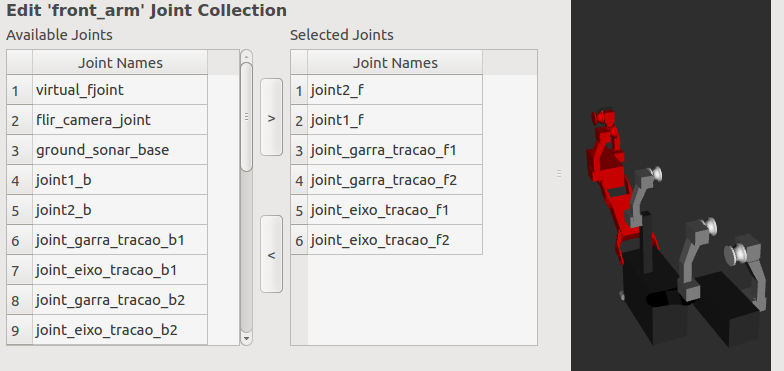
\includegraphics[width=1\textwidth]{planing_groups.png}
		\caption{Front Arm planning group from Elir Robot}
		\label{fig:plan_grp}
	\end{figure}

	\subsection{Robot Poses}
	Allows to set default robot poses,the figure \ref{fig:pose1} shows the default pose for the front arm when the robot is
	in the power line.
	
	\begin{figure}[h]
		\centering
		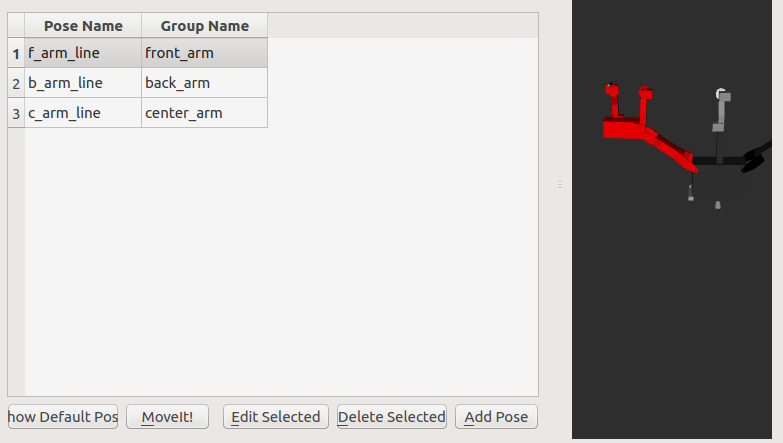
\includegraphics[width=.75\textwidth]{pose1.png}
		\caption{Front Arm pose from Elir Robot}
		\label{fig:pose1}
	\end{figure}
	
	\subsection{End-effector}
	The end effector configuration requires one end-effector group and one link to be the parent.
	There's an option of setting a parent group.
	
	\subsection{Passive Joints}
	The passive joints will specify joints that won't have their state published by MoveIT!, and they won't be considered in the motion planning. In the Elir Robot, in the first tests we will consider the \verb|joint-eixo-tracao| joints are passive.
	
	\subsection{Author Information}
	Author information for catkin purposes.
	
	\subsection{Generating Configuration Files}
	It Generates a catkin package with the configuration files needed to operate MoveIT!
	
	\section{Move Group Python Interface Tutorial}
	The move group launch file uses the  \verb|pr2_moveit_config/launch/demo.launch| ,it'll be necessary to create an rviz launch file, for the Elir Robot. 
	\bibliographystyle{plain}
	\bibliography{sample}


\end{document}

